\documentclass{article}
\usepackage{graphicx} % Required for inserting images
\usepackage{xcolor}
\usepackage{soul}
\usepackage{amsmath}

\title{Probability Theory and Linear Algebra}
\author{Benjamin "Benj1"}
\begin{document}
\maketitle
\section*{Lecture 1 - Introduction, vectors, linearity} 
\subsection*{Vectors}

%\textcolor{red}{Text colored with}
\hl{Vector is an ordered, finite list of numbers. Vectors are usually written as vertical arrays, surrounded by square or curved brackets:}
\section*{test}
\newline 
![Written vector example](/imgs/SLIAL/WrittenVector.png)

\newline 
\hl{They can also be written as numbers separated by commas and surrounded by parentheses. In this notation style, the vector above is written as: }

\newline 
%\begin{equation*}
	(−1.1, 0.0, 3.6, −7.2)
%\end{equation*}

\newline 
The elements (or entries, coefficients, components) of a vector are the values in the array. The size (also called dimension or length) of the vector is the number of
elements it contains. The vector above, for example, has size four; its third entry is 3.6. A vector of size *n* is called an *n-vector*. A 1-vector is considered to be the
same as a number, i.e., we do not distinguish between the 1-vector [ 1.3 ] and the number 1.3.
\newline 
We often use symbols to denote vectors. If we denote an *n-vector* using the symbol *a*, the *i*th element of the vector *a* is denoted *a_i*, where the subscript *i* is an integer index that runs from 1 to *n*, the size of the vector.
Two vectors *a* and *b* are *equal*, which we denote *a* = *b*, if they have the same size, and each of the corresponding entries is the same. If *a* and *b* are *n*-vectors, then *a* = *b* means *a*_1 = *b*_1, . . . , *a_n* = *b_n*.

\newline 
%\hl{The numbers or values of the elements in a vector are called scalars}. We will focus on the case that arises in most applications, where the scalars are real numbers. In this case we refer to vectors as real vectors. (Occasionally other types of scalars arise, for example, complex numbers, in which case we refer to the vector as a complex vector.) \hl{The set of all real numbers is written as **R**, and the set of all real *n*-vectors is denoted **R**^*n*}, so *a* ∈ **R**^*n* is another way to say that *a* is an *n*-vector with real entries. Here we use set notation: *a* ∈ **R**^*n* means that *a* is an element of the set **R**^*n*; see appendix A.

\newline 
**Block or stacked vectors.** It is sometimes useful to define vectors by *concatenating* or *stacking* two or more vectors, as in

\begin{figure}[H]
    \centering
    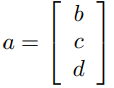
\includegraphics[width=0.4\textwidth]{imgs/SLIAL/StackedVectors.png}
    \caption{Block/Stacked bector example}
    \label{Block/Stacked bector example}
\end{figure}



![text](StackedVectors.png)

where *a*, *b*, *c*, and *d* are vectors. If *b* is an *m*-vector, *c* is an *n*-vector, and *d* is a
*p*-vector, this defines the (*m* + *n* + *p*)-vector
%\hl{The numbers or values of the elements in a vector are called scalars}. We will focus on the case that arises in most applications, where the scalars are real numbers. In this case we refer to vectors as real vectors. (Occasionally other types of scalars arise, for example, complex numbers, in which case we refer to the vector as a complex vector.) \hl{The set of all real numbers is written as **R**, and the set of all real *n*-vectors is denoted **R**^*n*}, so *a* ∈ **R**^*n* is another way to say that *a* is an *n*-vector with real entries. Here we use set notation: *a* ∈ **R**^*n* means that *a* is an element of the set **R**^*n*; see appendix A.
%\begin{equation*}
	*a* = (*b*_1, *b*_2, . . . , *b_m*, *c*_1, *c*_2, . . . , *c_n*, *d*_1, *d*_2, . . . , *d_p*)
%\end{equation*}.

\hl{The stacked vector *a* is also written as *a* = (*b*, *c*, *d*).}
Stacked vectors can include scalars (numbers). For example if *a* is a 3-vector,
(1, *a*) is the 4-vector (1, *a*_1, *a*_2, *a*_3).

**Subvectors.** In the equation above, we say that *b*, *c*, and *d* are *subvectors* or *slices* of *a*, with sizes *m*, *n*, and *p*, respectively. *Colon notation* is used to denote subvectors. If *a* is a vector, then the subvector *a_r:s* is a vector of size *s* − *r* + 1, with entries *a_r*, . . . , *a_s*:

\newline 
\newline 
\begin{equation*}
	*a_r*:*s* = (*a_r*, . . . , *a_s*)
\end{equation*}.

As a more concrete example, if \hl{*z* is the 4-vector (1, −1, 2, 0), the slice *z*_2:3 is *z*_2:3 = (−1, 2).} Colon notation is not completely standard, but is gaining traction.

\hl{In programming, arrays of length *n* are indexed from i = 0 to i = *n* − 1. In standard mathematical notation, *n*-vectors are indexed from i = 1 to i = *n*, so in this subject/class, vectors will be indexed from i = 1 to i = *n*}

**Zero vectors.** \hl{A *zero vector* is a vector with all elements equal to zero. Sometimes the zero vector of size *n* is written as 0_n, where the subscript denotes the size.But usually a zero vector is denoted just 0, the same symbol used to denote the number 0.</span> In this case you have to figure out the size of the zero vector from the context. As a simple example, if *a* is a 9-vector, and we are told that *a* = 0, the 0 vector on the right-hand side must be the one of size 9.
Even though zero vectors of different sizes are different vectors, we use the same symbol 0 to denote them. In computer programming this is called *overloading*: 
The symbol 0 is overloaded because it can mean different things depending on the context (e.g., the equation it appears in)

**Unit vectors.** \hl{A (standard) *unit vector* is a vector with all elements equal to zero, except one element which is equal to one. The *i*th unit vector (of size *n*) is the unit vector with *i*th element one, and denoted *e_i*.</span> For example, the vectors

![A standard unit vector](/imgs/SLIAL/StandardUnitvector.png)

are the three unit vectors of size 3. The notation for unit vectors is an example of the ambiguity in notation noted above. \hl{Here, *e_i* denotes the *i*th unit vector, and not the *i*th element of a vector *e*.</span> Thus we can describe the *i*th unit n-vector *e_i* as

![*i*th Unit Vector description](/imgs/SLIAL/ithUnitVectorDesc.png)

for *i,j* = 1, . . . , *n*. On the left-hand side *e_i* is an *n*-vector; (*e_i*)_*j* is a number, its *j*th entry. As with zero vectors, the size of *e_i* is usually determined from the context.

**Ones vector.** We use \hl{the notation **1**_*n* for the *n*-vector with all its elements equal to one. We also write **1** if the size of the vector can be determined from the context. (Some use *e* to denote a vector of all ones, but we will not use this notation.) The vector **1** is sometimes called the *ones vector*.</span>

**Sparsity.** \hl{A vector is said to be *sparse* if many of its entries are zero; its *sparsity pattern* is the set of indices of nonzero entries. The number of the nonzero entries of an *n*-vector *x* is denoted **nnz**(*x*). Unit vectors are sparse, since they have only one nonzero entry. The zero vector is the sparsest possible vector, since it has no nonzero entries.</span> Sparse vectors arise in many applications.

###

Literature: [VMLS], Chapter 1, Section 2.1 + slides
Exercises:

Basic vector notation and operations: 1.6, 1.7, 1.10, 1.11, 1.13
Block-vectors: 1.4
Linear combinations: 1.18
Linear functions: 2.1, 2.4
Affine functions: 2.2, 2.7
Regression models: 2.10, 2.12
Polynomials: 2.8

\section*{Lecture 1.5 - norm, distance, angle}

When: unscheduled!  Suggestion: 09.02.2004, afternoon.
Literature: [VMLS], Chapter 3

Exercises:
Properties of the norm: 3.3, 3.4, 3.18, 3.19
Nearest neighbour: 3.13
Angle: 3.22, 3.23
Chebyshev inequality: 3.7, 3.8
Block-vectors: 3.2

\section*{Lecture 2 - Linear independence}

Literature: [VMLS], Chapter 5 + Slides

Exercises:

Linear (in)dependence: 5.2, 5.1
Pythagoras theorem: 5.4
Orthognalization and Gram-Schmidt: 5.5-5.9
(facit -> moodle)

\section*{Lecture 3 - Matrices}
\h1{A matrix is a rectangular array of numbers written between rectangular brackets, as in}

\begin{bmatrix}
    0 & 1 & -2.3 & 0.1\\
    1.3 & 4 & -0.1 & 0\\
    4.1 & -1 & 0 & 1.7
\end{bmatrix}

It is also common to use large parentheses instead of rectangular brackets, as in

\begin{pmatrix}
    0 & 1 & -2.3 & 0.1\\
    1.3 & 4 & -0.1 & 0\\
    4.1 & -1 & 0 & 1.7
\end{pmatrix}

\h1{An important attribute of a matrix is its \textit{size} or \textit{dimensions} i.e, the numbers
of rows and columns.} The matrix above has 3 rows and 4 columns, so its size is 3 x 4.\newline
A matrix of size $m x n$ is called an $m x n$ matrix.\newline
The \textit{elements} (or \textit{entries} or \textit{coefficients}) of a matrix are the values in the array.\newline
The $i,j$ element is the value of the \textit{i}th row and \textit{j}th column, denoted by double subscripts:
the $i,j$ element of a matrix $A$ is denoted $A_ij$ (or $A_i,j$, when \textit{i} or \textit{j} is more than one digit or character).\newline
The positive integers \textit{i} and \textit{j} are called \textit{indices}. \newline
If $A$ is an $m x n$ matrix, then the row index runs from 1 to $m$ and the column index $j$ runs from 1 to $n$.
Row indices go from top to bottom, so row 1 is the top row, and row $m$ is the bottom row. Column indices go from left to right, so column
1 is the left column, and column $n$ is the right column.\newline
If the matrix above is $B$, then we have $B_13 = -2.3, B_32 = -1.$ the row index of the bottom left element (which has value 4.1) is 3;
its column index is 1.\newline
\h1{Two matrices are equal, if they have the same size, and if all the corresponding entries are equal.}\newline
As with vectors, we normally deal with matrices with entries that are real numbers, which will be our assumption unless stated otherwise.
\h1{The set of real $m x n matrices is denoted \textbf{R}^mxn$}. But matrices with complex entries, for example, do arise in some applications
\newline\newline
\textbf{Matrix indexing.} As with vectors, we in math index from 1. In computer langauges, a matrix is typically stored as a 2D array, where we would index the matrix from 0 (unless you use a package that index from 1). 
\newline\newline
\textbf{Square, tall and wide matrices.} A \textiit{sqare} matrix has an equal number of rows and columns. A square matrix of size $n x n$ is said to be of \textit{order} $n$.
A \textit{tall} matrix has more rrows than columns (size $m x n$ with $m > n$). A \textit{wide} matrix has more columns that rows (size $m x n$ with $n > m$).
\newline\newline
\textbf{Column and row vectors.} An \textit{n}-vectors

Literature: [VMLS], Chapters 6,7 + Slides

Exercises:
Dimensions: 6.1, 6.3
Matrix-vector multiplication: 6.6, 6.10, 6.11
Graph adjacency/incidence matrices: 6.4, 6.5, 7.7
Linear (in)dependence: 6.17, 7.6
Skew-symmetric matrices: 6.12
Various transformations: 6.13, 7.2, 7.3, 7.4, 7.8, 7.11
Complexity of matrix-vector product: 6.20
Norm of matrix-vector product: 6.14

\section*{Lecture 4 - Linear equations. Gaussian elimination}

This lecture is about vector-valued linear and affine functions, and systems of linear equations

\subsection*{Linear and affine functions}

**Vector-valued functions of vectors.** \hl{The notation *f* : R^n -> R^m means that *f* is a function that maps real *n*-vectors to real *m*-vectors.</span> The value of the function *f*, evaluated at an *n*-vector *x*, is an *m*-vector *f*(*x*) = (*f*_1(*x*), *f*_22(*x*),..., *f*_*m*(*x*)). Each of the components *f*_*i* of *f* is itself a scalar-valued function of *x*. As with scalar-valued functions, we sometimes write *f_i*(*x*) = *f_i*(*x*_1 *x*_2 *x_n*) to emphasize that *f* is a function of *n* scalar arguments. We use the same notation for each of the components of *f*, writing *f_i*(*x*) = *f_i*(*x*_1, *x*_2, ..., *x_n*) to emphasize that *f_i* is a function mapping the scalar arguments *x*_1, ..., *x_n* into a scalar.

**The matrix-vector product function.** \hl{Suppose *A* is an *m* X *n* matrix. We can define a function *f* : **R**^*n* -> **R**^*m* by *f*(*x*) = *Ax*. The inner product function *f* : **R**^*n* -> **R**, defined as *f*(*x*) = *a*^*T*_*x*, discussed in Lecture 1, is the special case with *m*=1.</span>

**Superposition and linearity.** The function *f*: *R^n* -> *R^m*, defined by *f*(*x*) = *Ax*, is *linear*, *i.e.*, it satisfies the superposition property:

![Superposition Property](/imgs/SLIAL/SuperpositionProperty.png)

holds for all n-vectors x and y and all scalars \alpha and \beta . It is a good exercise to parse this simple looking equation, since it involves overloading of notation. On the left-hand side, the scalar-vector multiplications \alpha x and \beta y involve *n*-vectors, and the sum \alpha x+\beta y is the sum of two *n*-vectors. The function *f* maps *n*-vectors to *m*-vectors, so *f*(\alpha x+\beta y) is an *m*-vector. On the right-hand side, the scalar-vector multiplications and the sum are those for *m*-vectors. Finally, the equality sign is equality between two *m*-vectors.

\hl{We can verify that superposition holds for *f* using properties of matrix-vector and scalar-vector multiplication:</span>

![Verify that superposition holds for *f*](/imgs/SLIAL/SuperpositionHolds.png)

\hl{Thus we can associate with every matrix *A* a linear function *f*(*x*) = *Ax*.
The converse is also true.</span> Suppose *f* is a function that maps *n*-vectors to *m*-vectors, and is linear, i.e., (8.1) holds for all *n*-vectors *x* and *y* and all scalars \alpha and \beta . Then there exists an *m* x *n* matrix A such that f(x) = Ax for all x. This can be shown in the same way as for scalar-valued functions in 2.1, by showing that if f is linear, then

![8.2](/imgs/SLIAL/8.2.png)

where *e_k* is the *k*th unit vector of size *n*. The right-hand side can also be written as a matrix-vector product *Ax*, with

![8.2.1](/imgs/SLIAL/8.2.1.png)

**Examples of linear functions.**

![Examples of linear functions](/imgs/SLIAL/ExamplesLinearFunctions.png)
![Examples of linear functions 2](/imgs/SLIAL/ExamplesLinearFunctions2.png)

**Examples of functions that are not linear** here we list some examples of functions *f* that map *n*-vectors x to n-vectors f(x) that are not linear. In each case
we show a superposition counterexample.

![Examples of nonlinear functions](/imgs/SLIAL/ExamplesNonlinearFunctions.png)

**Affine functions.** \hl{A vector-valued function *f* : **R**^*n* → **R**^*m* is called affine if it can be expressed as *f*(*x*) = *Ax* + *b*, where *A* is an *m × n* matrix and *b* is an *m*-vector. It can be shown that a function *f* : **R**^*n* → **R**^*m* is affine if and only if</span>

*f*(*α*x + *β*y) = *αf*(*x*) + *βf*(*y*)

holds for all *n*-vectors *x*, *y*, and all scalars *α*, *β* that satisfy *α* + *β* = 1. In other words, superposition holds for affine combinations of vectors. (For linear functions, superposition holds for any linear combinations of vectors.) 
The matrix *A* and the vector *b* in the representation of an affine function as *f*(*x*) = *Ax* + *b* are unique. These parameters can be obtained by evaluating *f* at the vectors 0, *e*_1, . . . , *e*_n, where *e_ k* is the *k*th unit vector in **R**^*n*. We have

A = [*f*(*e*_1) − *f*(0) *f*(*e*_2) − *f*(0) ... *f*(*e_n*) − *f*(0)], *b* = *f*(0).

Just like affine scalar-valued functions, affine vector-valued functions are often called linear, even though they are linear only when the vector *b* is zero.

**Linear function models**

\subsection*{Linear function models}

Many functions or relations between variables that arise in natural science, engineering, and social sciences can be approximated as linear or affine functions. In these cases we refer to the linear function relating the two sets of variables as a model or an approximation, to remind us that the relation is only an approximation, and not exact.

**Taylor approximation**
Suppose *f* : **R**^*n* → **R**^*m* is differentiable, i.e., has partial derivatives, and *z* is an *n*-vector. The first-order Taylor approximation of *f* near *z* is given by

![First-order Taylor approximation](/imgs/SLIAL/FirstOrderTaylorApproximation.png)

for *i* = 1, ..., *m*. (This is just the first-order Taylor approximation of each of the scalar-valued functions *f_i*, described in Lecture One.) For *x* near *z*, \hat{f}(*x*) is a very good approximation of *f*(*x*). We can express this approximation in compact notation, using matrix-vector multiplication, as

![Taylor approximation using compact notation](/imgs/SLIAL/TaylorApproximationCompactNotation.png)

where the *m* × *n* matrix D*f*(*z*) is the *derivative* or *Jacobian* matrix of *f* at *z* (see §C.1). Its components are the partial derivatives of *f*,

![Derivative or Jacobian matrix](/imgs/SLIAL/JacobianMatrix.png)

\hl{As in the scalar-valued case, Taylor approximation is sometimes written with a second argument as \hat{f}(*x*; *z*) to show the point z around which the approximation is made. Evidently the Taylor series approximation \hat{f} is an affine function of *x*. (It is often called a linear approximation of *f*, even though it is not, in general, a linear function.) </span>

\subsection*{Regression model}

Taking the regression model:

![The regression model](/imgs/SLIAL/RegressionModel.png)

where \hl{the *n*-vector *x* is a feature vector for some object, *β* is an *n*-vector of weights, *v* is a constant (the offset), and \hat{y} is the (scalar) value of the regression model prediction.
Now suppose we have a set of *N* objects (also called *samples* or *examples*), with feature vectors *x*^(1), ... , *x*^(N). The regression model predictions associated with the examples are given by</span>

![The regression model predictions associated with given examples](/imgs/SLIAL/RegressionModelPredictions.png)

These numbers usually correspond to predictions of the value of the outputs or responses. If in addition to the example feature vectors *x*^(*i*) we are also given the actual value of the associated response variables, *y*^(1), ..., *y*^(*N*), then our *prediction errors* or *residuals* are

![Regression model prediction errors (residuals)](/imgs/SLIAL/RegressionModelResiduals.png)

Literature: [VMLS], Chapter 8 + slides. You may find a much more detailed explanation of row reduction with examples in Sections 1.1-1.2 of [Lay]="Linear Algebra and Its Applications" by Lay, Lay, McDonald (attached). Note: I only discuss the (non-unique) echelon form in my slides, after which we run a backward substitution algorithm, whereas Lay also talks about the reduced echelon form. Basically we do not explicitly perform "Step 5" of the reduction algorithm on p. 17 in Lay's book.

Exercises:

[VMLS]: 8.1, 8.3, 8.4, 8.6, 8.8, 8.9, 8.14, 8.16
[Lay]: 1.1.1, 1.1.6. Run backward substitution: 1.1.7, 1.1.9. Determine consistency: 1.1.15, 1.1.17. Find all solutions to the system: 1.2.7, 1.2.9, 1.2.11, 1.2.13. Existence/uniqueness: 1.2.15, 1.2.19

\section*{Lecture 4.5 - matrix multiplication}

Literature: [VMLS], Chapter 10

Exercises:

Matrix multiplication: 10.1, 10.2, 10.3, 10.4, 10.6, 10.8, 10.12, 10.14, 10.23, 10.25, 10.26, 10.33, 10.34
Orthogonal matrices: 10.35, 10.38, 10.40 (there is an obvious typo in the definition of Qi)
Computational complexity: 10.42, 10.43, 10.44

\section*{Lecture 5 - Workshop 01}

When: 27.02.2024, 12:30

\section*{Lecture 6 - Matrix inverses}


\subsection*{Left and right inverses}
Recall that for a number a, its (multiplicative) inverse is the number x for which
xa = 1, which we usually denote as `*x* = 1/*a*` or (less frequently) `*x* = *a*^−1`. The inverse *x* exists provided *a* is nonzero. For matrices the concept of inverse is more complicated than for scalars; in the general case, we need to distinguish between left and right inverses. We start with the left inverse.

**Left inverse.** A matrix *X* that satisfies 
*X A* = *I*
is called a *left inverse* of A. The matrix *A* is said to be *left-invertible* if a left inverse exists. Note that if *A* has size *m × n*, a left inverse *X* will have size *n × m*,
the same dimensions as *A^T*


Literature: [VMLS], Chapter 11 + Slides

Exercises:

11.1, 11.2, 11.3, 11.4, 11.7, 11.12, 11.16, 11.17, 11.18, 11.22, 11.24
Block-matrices: 11.5 (hint: show that the inverse matrix is also symmetric; assume it has the same block-structure as A
), 11.6

\section*{Lecture 7 - Least-squares problems}

When: 08.03.2024, 12:30. This is a self-study with help.
Literature: [VMLS], Chapter 12 + slides

Exercises:

12.1, 12.2, 12.4, 12.9, 12.14, 12.16, 13.3

\section*{Lecture 8 - Workshop 02}

When: 12.03.2024, 12:30

\section*{Lecture 9 - Introduction, optimality conditions}

When: 18.03.2024, 10:15. Lecture followed up by exercises.
Literature: [AEP], from chapter 7 up to and including section 8.2.2 (pp 197-214) + section 10.2 (up and including Theorem 10.6 w/o proof, pp 243-248).

Exercises (from chapter9_exercises.pdf, see below). I recommend solving the practice problem, and at least a couple of exercises from each category besides "modelling". If you have time, please also look at the modelling exercises.

Solve the practice problems 1-4 on p.532
Solve graphically: exercises 9.2.7-9.2.10. I recommend trying to solve both the minimization and the maximization problem for each exercise.
Rewrite to standard, not canonical form: exercises 9.2.3-9.2.6. Randomize each problem by: randomly selecting minimize/maximize; then for each constraint randomly select from =
, ≤
, and ≥
; finally for each of the variables randomly select, whether it should be ≥0
, ≤0
, or "free"/no sign restrictied.
Duality: for each problem you stated in the standard form in the previous category, formulate the dual problem.
Modelling: exercises 9.2.1-9.2.2, 9.2.15.

\section*{Lecture 10 - Duality in linear optimization}

When: 22.03.2024, 12:30. This is a self-study with help.
Literature: [AEP], from chapter 7 up to and including section 8.2.2 (pp 197-214) + section 10.2 (up and including Theorem 10.6 w/o proof, pp 243-248).

Exercises (from chapter9_exercises.pdf, see below). I recommend solving the practice problem, and at least a couple of exercises from each category besides "modelling". If you have time, please also look at the modelling exercises.

Solve the practice problems 1-4 on p.532
Solve graphically: exercises 9.2.7-9.2.10. I recommend trying to solve both the minimization and the maximization problem for each exercise.
Rewrite to standard, not canonical form: exercises 9.2.3-9.2.6. Randomize each problem by: randomly selecting minimize/maximize; then for each constraint randomly select from =
, ≤
, and ≥
; finally for each of the variables randomly select, whether it should be ≥0
, ≤0
, or "free"/no sign restrictied.
Duality: for each problem you stated in the standard form in the previous category, formulate the dual problem.
Modelling: exercises 9.2.1-9.2.2, 9.2.15.

\section*{Lecture 11 - Simplex algorithm}

When: 26.03.2024, 12:30. This is a self-study with help.
Literature: [AEP]: Section 8.2.2 up to Theorem 8.7 (you do not have to read the proof)+Chapter 9.

Exercises:

Go through the full solutions of example1 (only Phase II) and example 2 (Phase I + II) on moodle
[AEP]: Exercises 9.1, 9.2(a)
Exercises from [chapter9_exercises], section 9.3: 9-14, 1-2.  Ignore everything about the "simplex tableau", just use simplex method to solve the problems (after reformulating them in standard form).
[AEP]: 8.6

\section*{Lecture 12 - Workshop 03}

When: 04.04.2024, 12:30.

\section*{Lecture 13 - Introduction to probability theory}

When: 09.04.2024, 12:30. Lecture followed up by exercises.
Literature: [Rosen] Sections 7.1-7.2

Exercises:

Compute the probabilities [7.1]: 3, 7, 9, 11
Compare the probabilities [7.1]: 37, 45
Probability distributions [7.2]: 1, 3, 5

\section*{Lecture 13.5 - mean value, variance}

When: unscheduled! Suggestion: 12.04.2024, afternoon
Literature: [Rosen] Section 7.4 + slides

Exercises:

Compute the expected value: [7.4] 3, 5, 7, 11
Independence: [7.4] 19, 21
Variance: [7.4] 27, 29

\section*{Lecture 14 - Conditional probability. Bayes' theorem}

When: 16.04.2024, 12:30. This is a self-study with help.
Literature: [Rosen], Sections 7.2-7.3 + slides

Exercises:

Compute the probabilities: [7.2] 7, 10, 29, 30
Conditional probabilities: [7.2] 23, 24, 25
Independent events: [7.2] 26, 27
Bernoulli trials: [7.2] 34, 35
Bayes' thm: [7.3]: 1, 3, 5, 9, 13, 15, 23

\section*{Lecture 14.5 - eigenvalues and eigenvectors}

When: unscheduled! Suggestion: 19.04.2024, afternoon
Literature: Section 5.1 of [Lay]="Linear Algebra and Its Applications" by Lay, Lay, McDonald (attached) + slides. Lay gives the definitions and explains the way of computing eigenvectors given the knowledge of an eigenvalue. QR (and other) algorithms are used in practice to compute eigenvalues.

Exercises:

[Lay]: 5.1.2, 5.1.5, 5.1.7, 5.1.17, 5.1.19, 5.1.21

\section*{Lecture 15 - Linear dynamical systems, Markov chains}

When: 23.04.2024, 12:30. This is a self-study with help.
Literature: [Lay], Section 4.9 + slides. Skim through [VMLS], Chapter 9 for some examples/applications

Exercises:

[Lay 4.9]: 1, 11, 7, 9, 10, 19, 20. Use QR algorithm to approximate the matrix eigenvalues in the exercise 7.
[VLMS]: 9.4, 9.3

\section*{Lecture 16 - Workshop 04}

When: 30.04.2024, 12:30.

\section*{Other notes:}
## Reduction
Remember, in order to isolate a variable:
![Isolating variable](/imgs/SLIAL/IsolatingAVariable.png)

\end{document}